%\title{Hebrew document in WriteLatex - מסמך בעברית}
\documentclass[11pt]{article}
\usepackage[utf8x]{inputenc}
\usepackage[english,hebrew]{babel}
\selectlanguage{hebrew}
\usepackage[top=1cm,bottom=1cm,left=2.5cm,right=2cm]{geometry}
\linespread{1.3} 
\usepackage{graphicx}
\usepackage{wrapfig}
\usepackage{caption}
\usepackage{subcaption}
\usepackage{indentfirst}
\title{%
\small
המכללה האקדמית להנדסה ע"ש סמי שמעון \L{SCE}, באר שבע\\ \vspace{+1em}
\Large
מודל לזיהוי אוטומטי שלד
הגדרות מתמטיות בטקסט
חופשי\\
\L{BS\_SE-18-23}\vspace{-3.5em}}
\date{}

\begin{document}
\maketitle
\selectlanguage{english}
\begin{figure}[h]
   \centering
   %
\includegraphics[height=30mm, width=25mm]{pic1.jpg}\hspace{1cm}
   %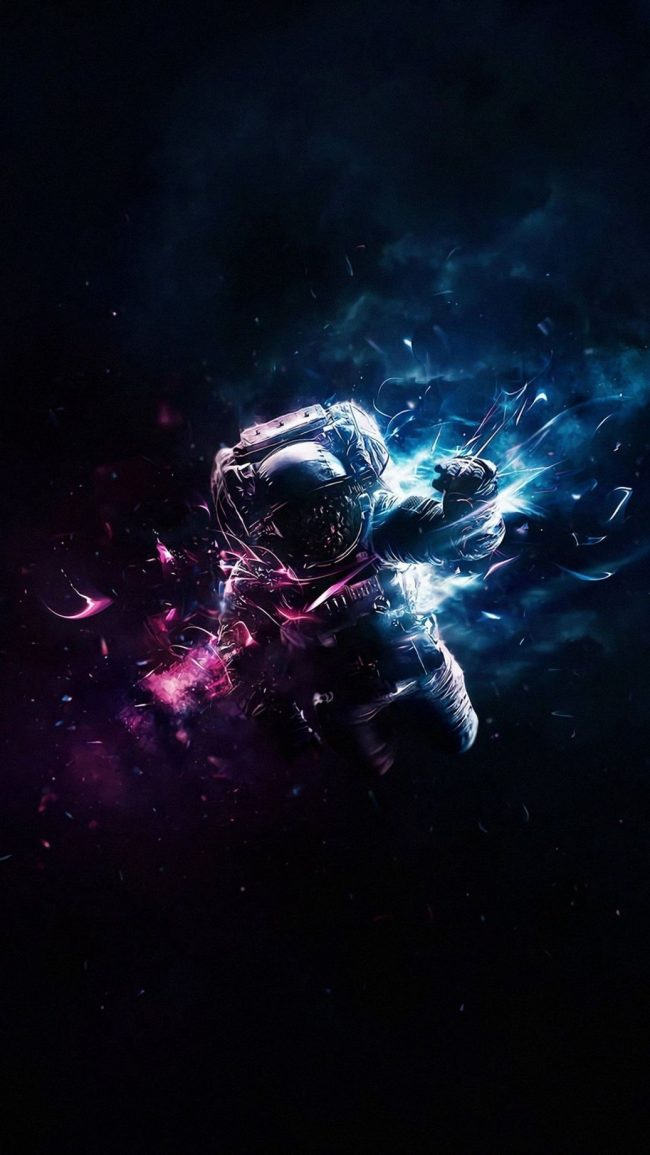
\includegraphics[height=30mm, width=25mm]{pic2.jpg}
   
    \begin{subfigure}[b]{0.31\textwidth}
        \centering
        
\includegraphics[height=40mm, width=35mm]{pic1.jpg}
        \\     {\R{שם מלא}\\ localPart@ac.sce.ac.il}
    \end{subfigure}
    \quad
    \begin{subfigure}[b]{0.31\textwidth} 
        \centering 
        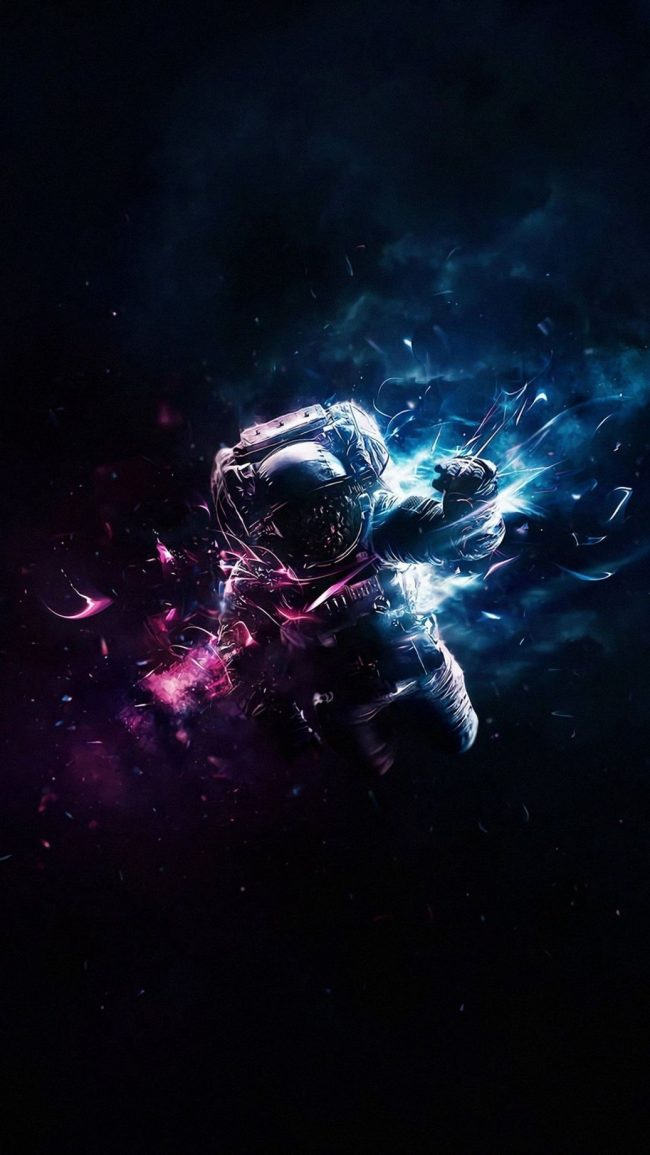
\includegraphics[height=40mm, width=35mm]{pic2.jpg}
        \caption*{\R{שם מלא}\\ localPart@ac.sce.ac.il}
    \end{subfigure}
    \quad
    \begin{subfigure}[b]{0.31\textwidth} 
        \centering 
        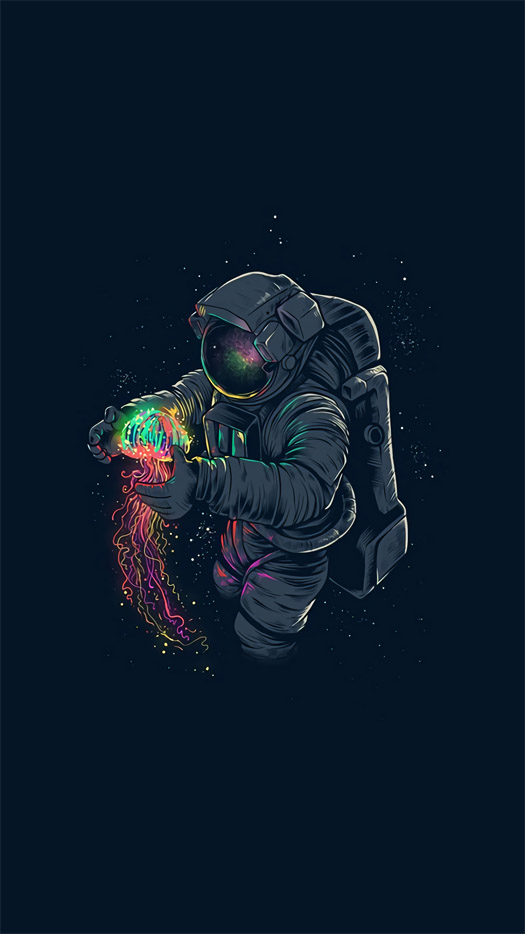
\includegraphics[height=40mm, width=35mm]{pic3.jpg}
        \caption*{\R{שם מלא}\\ localPart@ac.sce.ac.il}
    \end{subfigure}
\end{figure}
\thispagestyle{empty}

\selectlanguage{hebrew}
\subsubsection*{מנחה/ים:}
\section*{תקציר}

זוהי הפסקה בעבריתבמשך מאות שנים בני אדם בנו תבניות ודפוסים בניתוח מידע, אולם הצמיחה בנפח המידע בזמן
המודרני הגבירה את הצורך בגישות אוטומטיות יותר. אחד הגישות העוזרת לנתח וללמוד מהמידע
היא בינה מלאכותית \L{(Artificial Intelligence)}. 
הפרויקט שלנו הולך להתמקד בחלק הקטן של
בינה מלאכותית – למידה עמוקה \L{(Deep Learning )}.
לידע בזיהוי אוטומטי של הגדרות ישנה חשיבות רבה בשילוב עם יישומים, הרכבת אוטומטית של
מילונים, טקסונומיה, בעיית תשובות לשאלות, חיפוש סמנטי. בהכללה ניתן להציג את זיהוי אוטומטי
של הגדרות כבעיית סיווג של משפטים של הגדרה ולא.
בפרויקט זה אנחנו מציגים את המחקר שלנו רשתות נוירונים \L{CNN} ו \L{RNN} כאשר יכולת שלהם
שופרה על ידי הוספת ידע לשוני ותלויות בין המילים. הניסויים והתוצאות שלהם במשימת זיהוי
הגדרות נבנו לפי שלושה מערכי מידע \L{WCL} , \L{W00} , \L{Wolfram} .
הוספנו את \L{dataset} חדש שמורכב ממשפטים עם ניסוח מתמטי כדי להתמודד עם זיהוי אוטומטי של
הגדרות מתמטיות.
מערכת שלנו בונה מודלים ומאמנת אותם לפי קריטריונים שמשתמש מגדיר. משתמש יכול לבנות
מודל שונה בעזרת יצירה או הרחבה של מערכי מידע הנתונים.
משתמש יכול לשלב את המודלים שלנו בעבודות מחקר שונים ולהפעיל פונקציונליות של המודלים.
במהלך הפרויקט תוצאות והשוות למערכות אחרות. נצפה שיפור ניכר על ידי הוספת \L{dataset}
שיצרנו.

\subsubsection*{מילות מפתח:}
\end{document}